%
%
%

\documentclass[manuscript,anonymous,review]{acmart}
% \documentclass[manuscript,screen,review]{acmart}

\usepackage{here} % [H]とするとその場所に配置されるらしい

\def\HL{\textsf{HelpLine}}
\def\HF{\textsf{Helpfeel}}
\def\GIT{\texttt{git}}
\def\ES{\textsf{ExpandSearch}}
\def\SB{\textsf{Scrapbox}}
\long\def\tt#1{\texttt{#1}}
\long\def\stt#1{\texttt{\fontsize{8pt}{0pt}\selectfont{#1}}}
\long\def\sf#1{\textsf{#1}}
\long\def\ssf#1{\textsf{\fontsize{8pt}{0pt}\selectfont{#1}}}
\long\def\qtt#1{``\tt{#1}''}   % quote tt
\long\def\sqtt#1{``\stt{#1}''} % small quote tt
\long\def\qsf#1{``\sf{#1}''}
\long\def\sqsf#1{``\ssf{#1}''}
\long\def\qit#1{``\textit{#1}''}
\long\def\smallfont{\fontsize{8pt}{0pt}\selectfont}

\long\def\comment#1{}

%%
%% \BibTeX command to typeset BibTeX logo in the docs
\AtBeginDocument{%
  \providecommand\BibTeX{{%
    \normalfont B\kern-0.5em{\scshape i\kern-0.25em b}\kern-0.8em\TeX}}}

%% Rights management information.  This information is sent to you
%% when you complete the rights form.  These commands have SAMPLE
%% values in them; it is your responsibility as an author to replace
%% the commands and values with those provided to you when you
%% complete the rights form.
\setcopyright{acmcopyright}
\copyrightyear{2020}
\acmYear{2020}
\acmDOI{10.1145/1122445.1122456}

%% These commands are for a PROCEEDINGS abstract or paper.
\acmConference[IUI '21]{IUI '21: ACM Conference}
  {June 03--05, 2020}{Somewhere, Italy}
\acmBooktitle{Woodstock '18: ACM Symposium on Neural Gaze Detection,
  June 03--05, 2018, Woodstock, NY}
\acmPrice{15.00}
\acmISBN{978-1-4503-XXXX-X/18/06}

%%
%% Submission ID.
%% Use this when submitting an article to a sponsored event. You'll
%% receive a unique submission ID from the organizers
%% of the event, and this ID should be used as the parameter to this command.
%%\acmSubmissionID{123-A56-BU3}

%%
%% The majority of ACM publications use numbered citations and
%% references.  The command \citestyle{authoryear} switches to the
%% "author year" style.
%%
%% If you are preparing content for an event
%% sponsored by ACM SIGGRAPH, you must use the "author year" style of
%% citations and references.
%% Uncommenting
%% the next command will enable that style.
%%\citestyle{acmauthoryear}

%%
%% end of the preamble, start of the body of the document source.
\begin{document}

%%
%% The "title" command has an optional parameter,
%% allowing the author to define a "short title" to be used in page headers.
\title{Beyond query expansion - expanding documents for fluid keyword search}

%%
%% The "author" command and its associated commands are used to define
%% the authors and their affiliations.
%% Of note is the shared affiliation of the first two authors, and the
%% "authornote" and "authornotemark" commands
%% used to denote shared contribution to the research.
\author{Toshiyuki Masui}
\email{masui@pitecan.com}
\orcid{1234-5678-9012}
\affiliation{%
  \institution{Keio University}
  \streetaddress{1234 Endo}
  \city{Fujisawa}
  \state{Kanagawa}
  \country{Japan}
  \postcode{43017-6221}
}

%%
%% By default, the full list of authors will be used in the page
%% headers. Often, this list is too long, and will overlap
%% other information printed in the page headers. This command allows
%% the author to define a more concise list
%% of authors' names for this purpose.
\renewcommand{\shortauthors}{Toshiyuki Masui}

%%
%% The abstract is a short summary of the work to be presented in the
%% article.
\begin{abstract}
  Although intelligent text search algorithms are widely available
  these days, searching documents is still difficult in many cases.
  It is
  usually hard to find useful information in help systems and manual
  pages, even when required information exists in the documents.

  Searches fail mainly because of the ``vocabulary problem,'' where users
  cannot find the right search keyword. When a user wants to
  ``remove a file,''and there is a manual entry or ``deleting a file,'' users may
  not be able to know how to remove a file until he finds the right
  keyword ``delete'' for the search.
  To solve the problem, various \textit{query expansion}
  techniques are widely used on the Web. When a user
  types ``remove'' in the search box, the system automatically expands the
  keyword and suggests using ``remove/delete'' instead. Query expansion
  works effectively for simple cases, but it does not work well when the
  concept in the users' mind is very different from the text in the
  manual document. For example, if a user wants to ``clean up the
  desktop,'' he cannot find an appropriate manual entry that only
  describes how to ``delete icons'' or ``align icons'' on the desktop.

  We propose a new approach \textit{document expansion} for finding
  help documents and manual entries. We provide flexible explanations
  for each document using regular expression patterns. For the above
  example, we give an expression like \texttt{(delete|remove) (a file|data)}
  and use the expanded text like \texttt{delete a file}, \texttt{remove data} for
  keyword search. Also, a pattern like \texttt{(delete|remove) \#{file}} is
  expanded to \texttt{delete Makefile}, \texttt{delete search.c}, etc. depending on
  the existing files, so that a user can enter \texttt{del ma} to get
  \texttt{delete Makefile} and immediately execute it.

  We have been using this document expansion technique called
  {\ES} for several years, and the system is working on various
  commercial Web services. In this paper, we describe the idea and
  implementation of {\ES} and show how it works in the wild.
\end{abstract}

% 異なる言語でも大丈夫
% Translation paradigm


%%
%% The code below is generated by the tool at http://dl.acm.org/ccs.cfm.
%% Please copy and paste the code instead of the example below.
%%
\begin{CCSXML}
<ccs2012>
 <concept>
  <concept_id>10010520.10010553.10010562</concept_id>
  <concept_desc>Computer systems organization~Embedded systems</concept_desc>
  <concept_significance>500</concept_significance>
 </concept>
 <concept>
  <concept_id>10010520.10010575.10010755</concept_id>
  <concept_desc>Computer systems organization~Redundancy</concept_desc>
  <concept_significance>300</concept_significance>
 </concept>
 <concept>
  <concept_id>10010520.10010553.10010554</concept_id>
  <concept_desc>Computer systems organization~Robotics</concept_desc>
  <concept_significance>100</concept_significance>
 </concept>
 <concept>
  <concept_id>10003033.10003083.10003095</concept_id>
  <concept_desc>Networks~Network reliability</concept_desc>
  <concept_significance>100</concept_significance>
 </concept>
</ccs2012>
\end{CCSXML}

\ccsdesc[500]{Computer systems organization~Embedded systems}
\ccsdesc[300]{Computer systems organization~Redundancy}
\ccsdesc{Computer systems organization~Robotics}
\ccsdesc[100]{Networks~Network reliability}

%%
%% Keywords. The author(s) should pick words that accurately describe
%% the work being presented. Separate the keywords with commas.
\keywords{text search, help systems, query expansion}


%%
%% This command processes the author and affiliation and title
%% information and builds the first part of the formatted document.
\maketitle

\section{Introduction}

People are frequently searching information using keywords on Google
and other systems.
But keyword search is still not an easy task,
because it is fundamentally difficulto to find appropriate information
that does not contain the keyword given by the user.

% Webでもパソコンでも情報検索はキーワード検索が主流だが、キーワード検索は昔も今も難しい
% 根本的に、[[本文に含まれていない文字列の検索が難しい]]からである

The standard help system on MacOS (Catalina v10.15.5)
cannot tell the user how to remove a file (Figure \ref{machelp}(a)).
%
It can tell the user how to ``set the clock'', but
the user has to know that
``setting the clock'' and ``changing date'' means the same thing (Figure \ref{machelp}(b)).

\begin{figure}[H]
  %\centering
  % 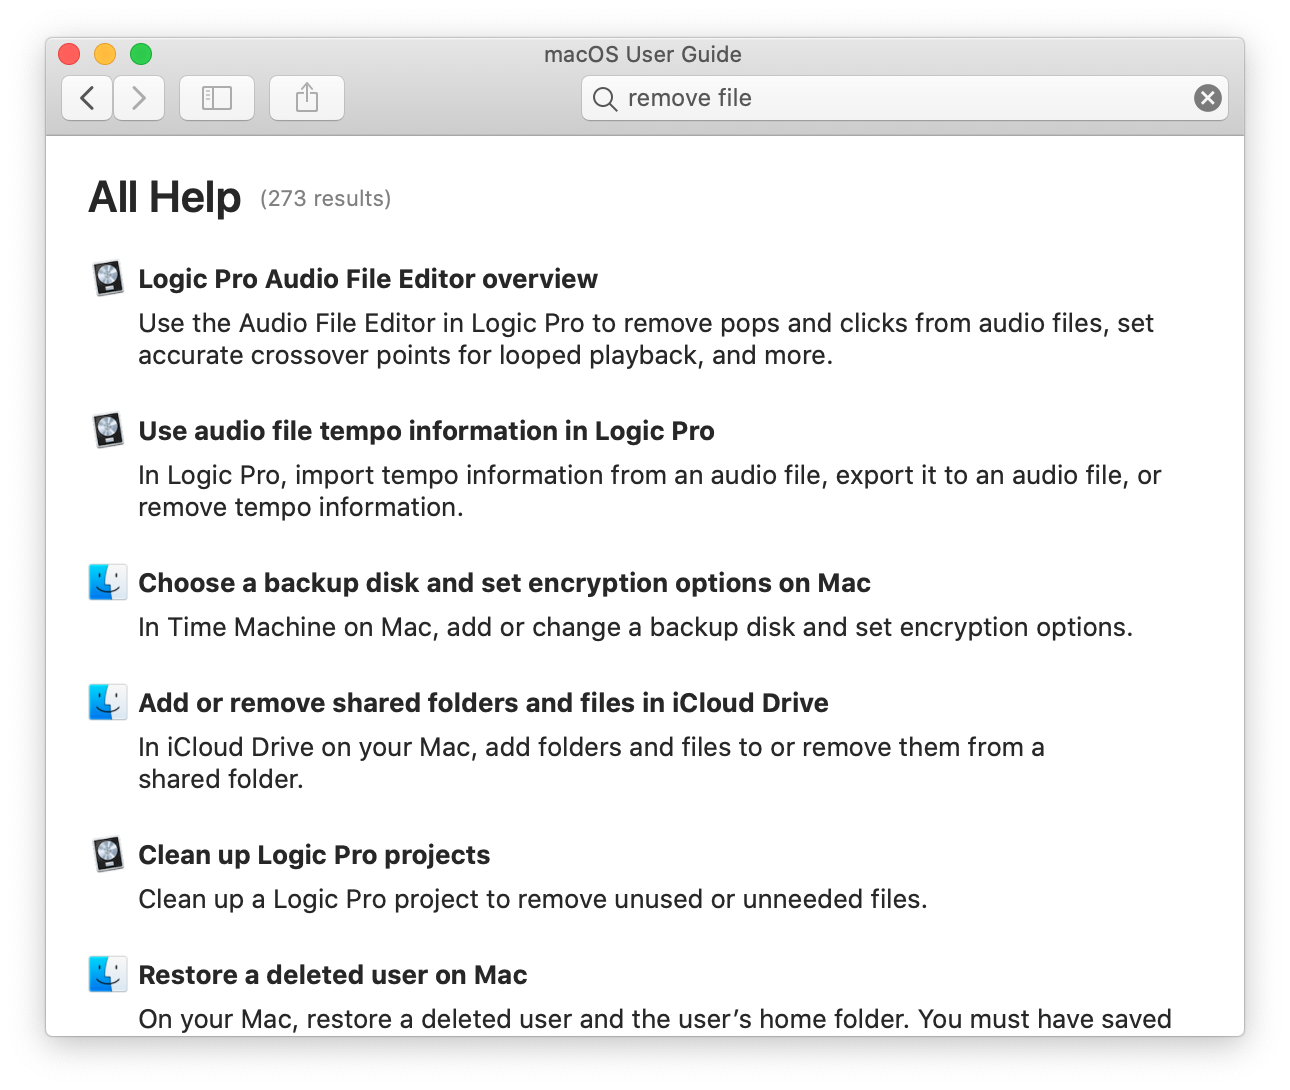
\includegraphics[width=7cm,bb=0 0 1290 1090]{figures/eaa80e41ddc3d3620fae133007274573.png}
  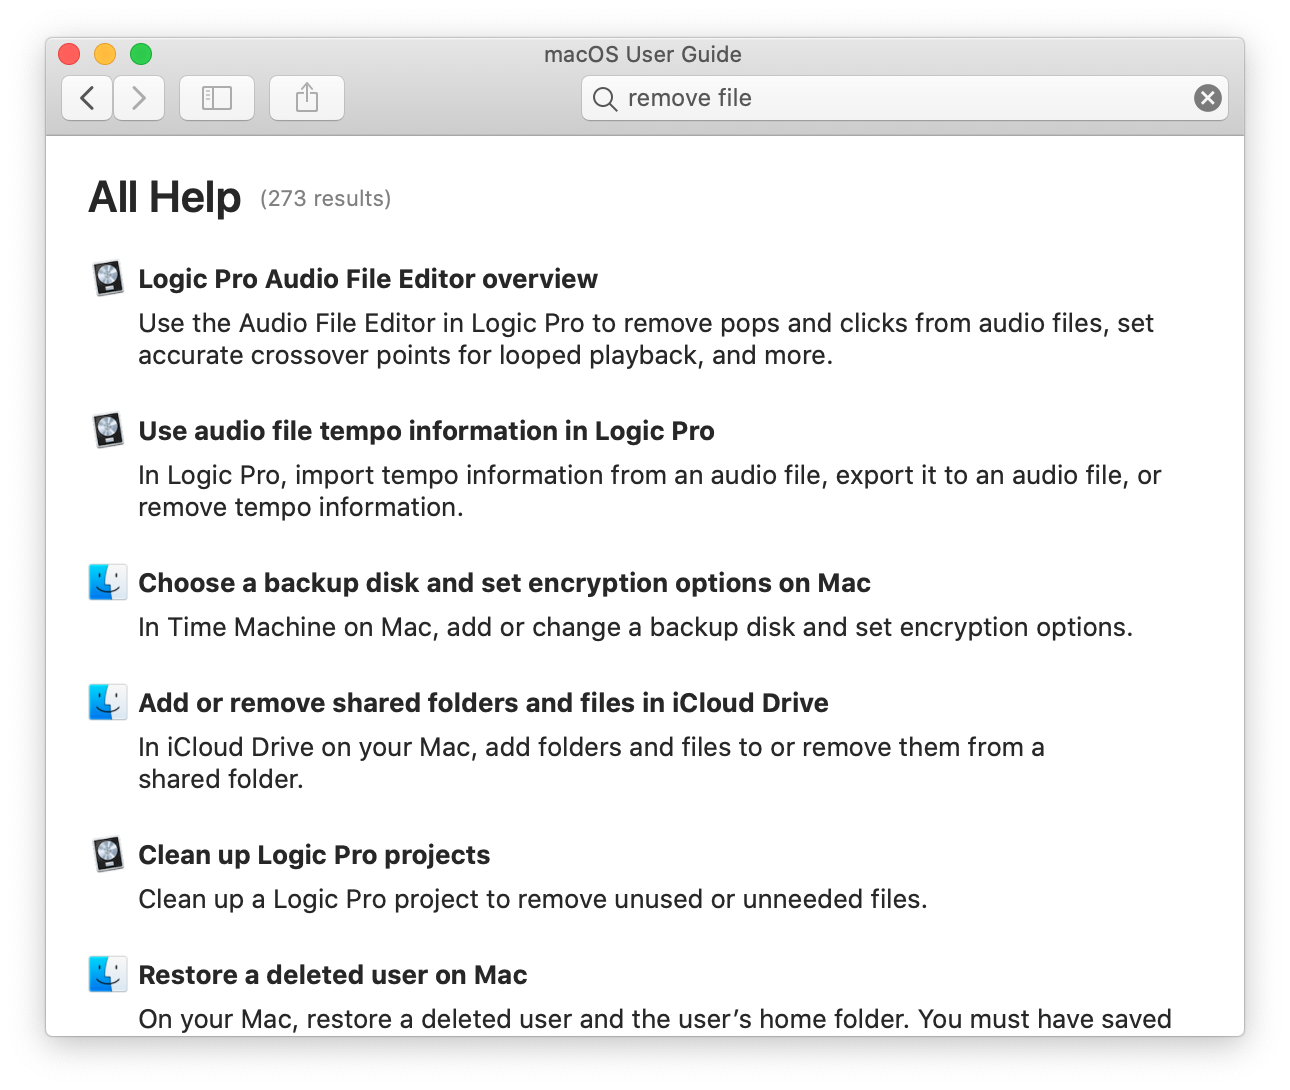
\includegraphics[width=7cm,bb=-50 0 950 800]{figures/eaa80e41ddc3d3620fae133007274573.png}
  % 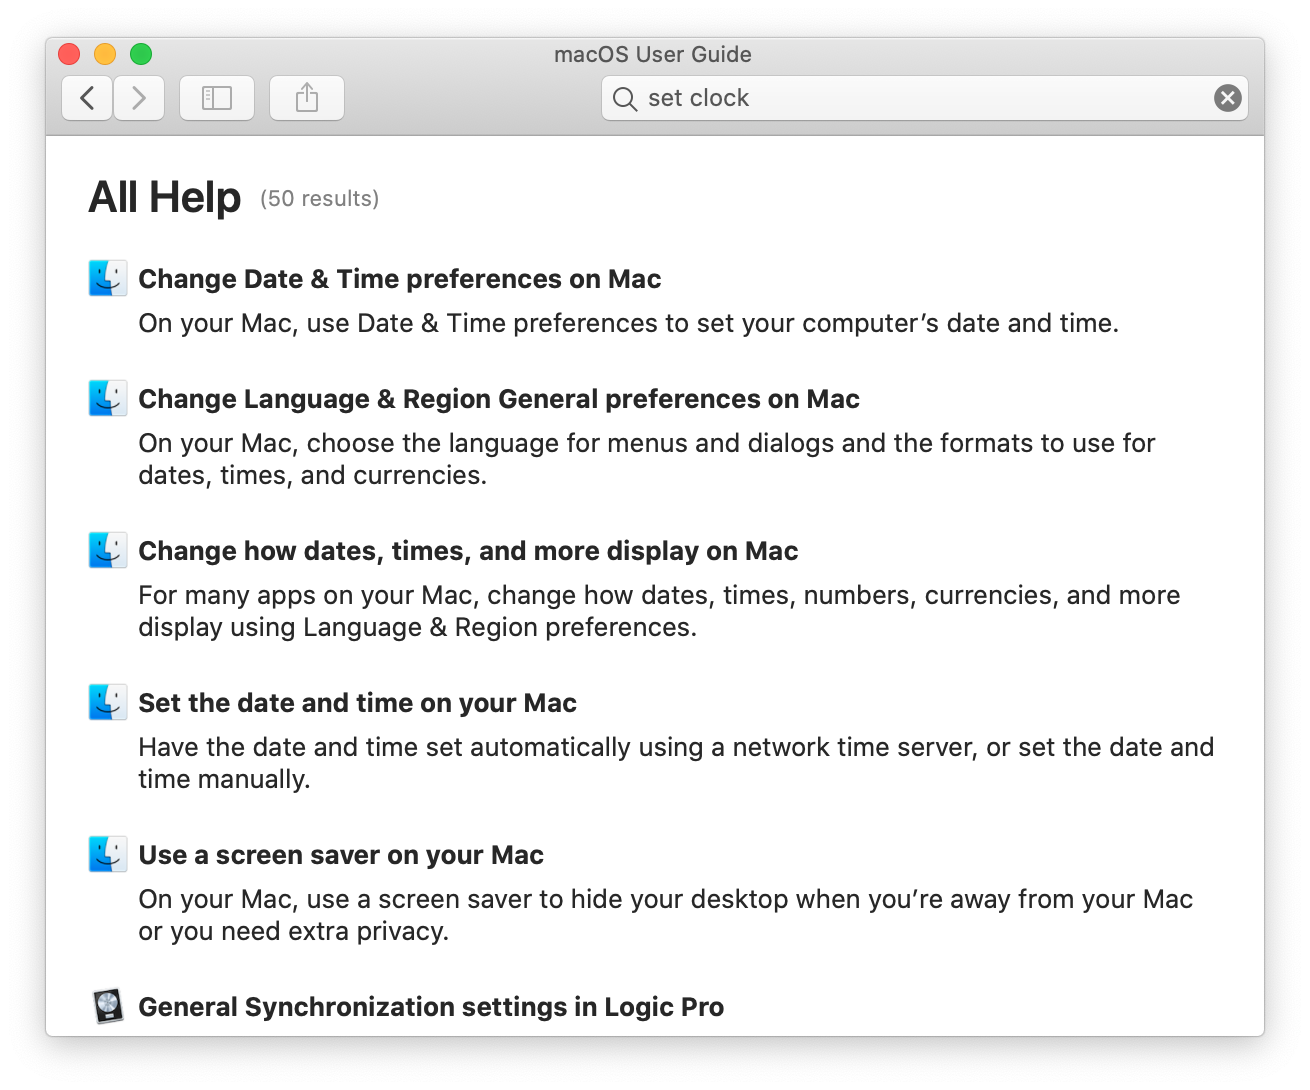
\includegraphics[width=7cm,bb=0 0 1310 1090]{figures/0cd679128d8f69eb2a8a966d6466a8a4.png}
  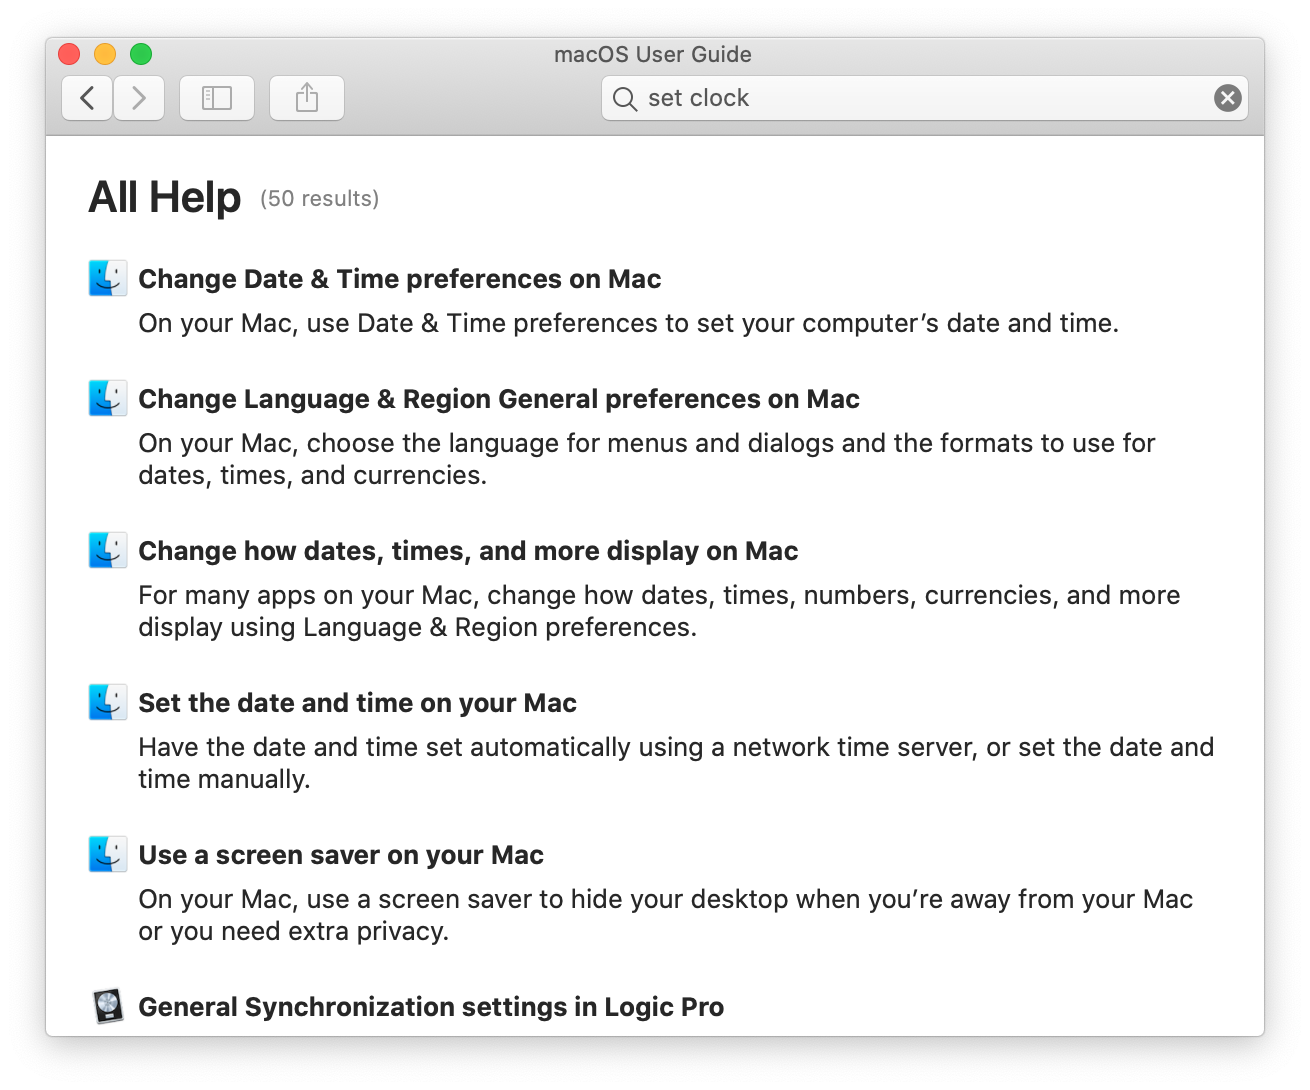
\includegraphics[width=7cm,bb=-50 0 950 800]{figures/0cd679128d8f69eb2a8a966d6466a8a4.png}
  \par
  (a) Searching ``remove files'' \hspace{3cm} (b) Searching ``Set clock''
  \caption{Using the standard help application on Mac.}
  \label{machelp}
  %\Description{Mac Mac}
\end{figure}

% \begin{figure}[H]
%   \centering
%   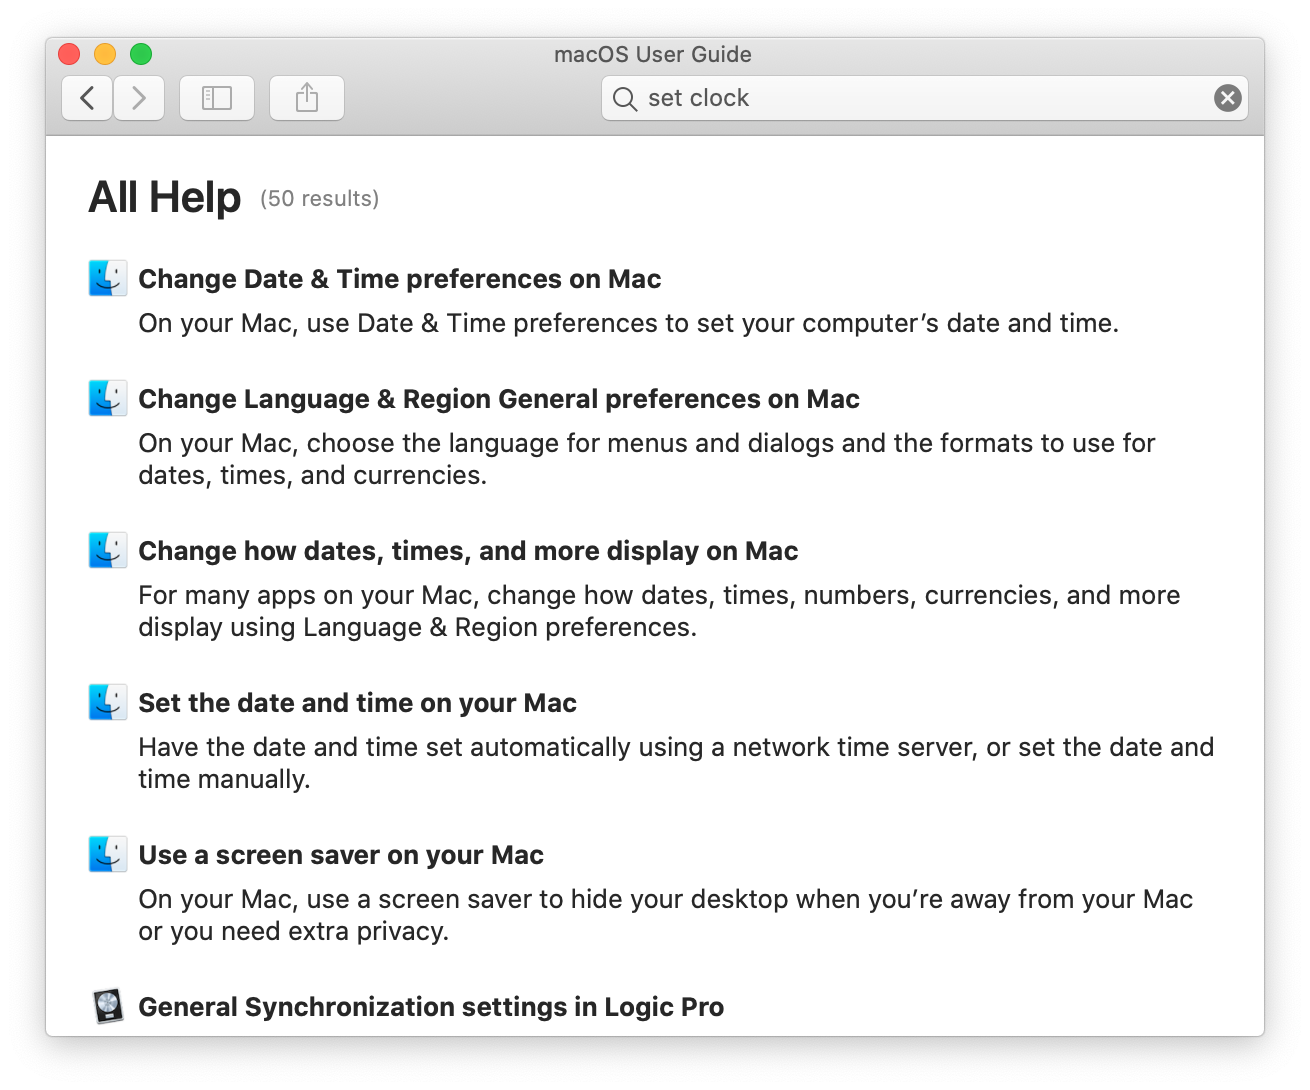
\includegraphics[width=12cm,bb=0 0 1310 1090]{figures/0cd679128d8f69eb2a8a966d6466a8a4.png}
%   \caption{Mac}
%   \Description{Mac Mac}
% \end{figure}

We can get this kind of information fairly easily using Google and other search engines on the net,
so many people prefer getting information on the net rather than
using help systems provided by manufacturers.

We can find information on Google because there are tremendous information
that describe how to ``remove a file'' on Mac.
If there are documens that contain ``remove'', ``file'', and ``Mac'',
finding such documents are not difficult.
That seems to be the main reason why people are satisfied with search engines
for finding popular information.

% For example we can find how to XXXX by using YYYY, because somebody on the net has written an article on XXXX using the keyword YYYY.

% Googleとかで意外とみつかる気がするのは、Web上のメジャーな情報は
% いろんな人がいろんな言葉で情報をアップしてるからだろう (出典)
% 機能を検索したとき、トップに出るのはメーカーのサイトではない
% 情報が無いからではなく、キーワードがマッチしないからだと思われる

On the other hand,
finding less popular information is more difficult,
because not enough documents related to the topic exist on the net.
%
If there is only one document on the net
that describes the \qtt{console} feature of a relatively minor system like \tt{Heroku},
people cannot find the document using a similar keyword \qtt{dashboard}
since the documents from \tt{Heroku} does not contain the word \qtt{dashboard}.

% メジャーじゃないシステムや特殊な状況のヘルプなどの場合、文書もユーザも少ないから苦労する
% キーワードが少しでも違うとみつからない
% 開発者の用語とユーザの用語が違うことの違いの問題がさらにひどい

% e.g. メジャーじゃないxxxxxシステムのyyyyy機能
%   Google Chrome Extensionのconsoleとかみつからない (dashboardだとみつかる)
% 	(他の例も)

FAQs (frequently asked questions) by manufacturers and service providers are
usually not considered useful
because the words used in the documents are
often different from the keywords that user can imagine.

% いわゆるFAQは大抵不十分(出典)
%   特殊なサービスの特殊な機能について書かれてることが多いからだろう
%   メジャーなサービスであっても、ググって本家FAQが出てくることなど無い
%    誰かが言い替えたものがヒットするのが普通 (出典)

Even finding the users' old memos can be sometimes difficult,
because people might use different keywords for the same thing case by case.
He might try to find a file related to ``IUI'' and fail, because he used
the term ``intelligent user interface'' for the file name.
%
Various techniques have been proposed to solve this vocabulary problem\cite{Furnas:1987:VPH:32206.32212},
but not very successful enough.

% 自分のメモですら後でみつけられなくて困ることも多い
%  微妙に利用単語が違うとみつからない
%  良いファイル名をつけたつもりでも後から検索できないことがある

Finding documents are even more difficult when
the user's mother language is different from the language used in the document.
When a user wants to find how to ``delete a file'' but the
manual of the system is written in French,
he has to \textit{translate} the term ``delete'' and ``file'' into French
before the search.
Non-English speakers are always having trouble
translating the word in their brain into English words
before searching information, because important information are
usually provided in English.

% 母語が違うときはさらに大変である
% 頭の中の単語を英語に変換する必要がある
% 常にTranslationや言い替えが必要だといっていいだろう
% (いったん文書がみつかれば、それを理解することはできるが、そもそもみつけるのが難しいのである)
% クエリや検索技術を工夫して解決しようとする方法が多い
% 原文はいじれないから
%  いろんな言い回しで検索する研究は大昔からある

\subsection*{Query Expansion}

% Query expansion (QE) is the process of reformulating a given query to
% improve retrieval performance in information retrieval operations,
% particularly in the context of query understanding.[1] In the context
% of search engines, query expansion involves evaluating a user's input
% (what words were typed into the search query area, and sometimes other
% types of data) and expanding the search query to match additional
% documents. Query expansion involves techniques such as:
% 
% * Finding synonyms of words, and searching for the synonyms as well
% * Finding semantically related words (e.g. antonyms, meronyms, hyponyms, hypernyms)
% * Finding all the various morphological forms of words by stemming each word in the search query
% * Fixing spelling errors and automatically searching for the corrected form or suggesting it in the results
% * Re-weighting the terms in the original query
%
% Query expansion is a methodology studied in the field of computer
% science, particularly within the realm of natural language processing
% and information retrieval.

The vocabulary problem and the translation problem can partially be solved
if the search system have a thesaurus and a translation dictionary.
%
For example, 
if the system knows that removing a file and deleting a file mean the same thing,
the system can try to find something using the keyword ``delete'',
even when the user specified the keyword ``remove''.
%
Techniques like this are called ``\textit{Query expansion}''\footnote{
  \ssf{https:{\slash}{\slash}en.wikipedia.org{\slash}wiki{\slash}Query\_expansion}
},
and simple query expansion is effective if a good thesaurus is available.

% クエリに工夫する方法
%    シソーラス的検索の一般化
%    検索対象の本文は変わらないから不十分
%    クエリだけ拡張してもしょうがない
%    本文に固有名詞的なものが少ない場合はみつけにくい
%    e.g. 「良い論文を書く方法」「査読を通す方法」「インパクトある論文を書く方法」
%     「レビュワーを説得する技術」 vs 「良い論文を書く方法」
% ユーザが指定するあらゆるキーワードを拡張するのは不可能である
% John F. Kennedy
% 
% 翻訳してから検索するのも一種のQUery Expansionである
% 日本語を入力すると英語のWikipediaがみつかることもある => これは違う原理

Query expansion is effective when simple substitution of keywords are satisfactory enough.
In the previous example, using the keyword ``delete'' in addition to ``remove'' works
for finding the manual entry.
More sophisticated query expansion techniques are widely used in various modern
information retrieval systems.

However, query expansion techniques do not work for finding a document for vague topics.
For example, if you want to find a document that describes ``how to write a good paper'',
you will have little chance finding a document related to the topic.
Maybe it would be better to use keywords like ``how to persuade reviewers''.
However, expanding a phrase like ``write a good paper'' to ``persude reviewers'' is impossible,
unless the expander understands the intension of the user.

%  別の言い替え文書(Tipsとか逆引き辞典)を用意
%   便利だがメジャーなものに限られる
%   もと文書と全然違うところで作り直しは大変すぎるが、逆引き本は売れている
%   hands-on と言うのだろうか?
%    ちょっと違う
%    handbook かな?
%    firsthand

% ライブラリ関数 (やめる)
% 「配列からランダムに要素をふたつ取得」 = `a.sample(2)`
%    `sample`という単語はなかなか出てこないのではないか
%    pick upとかselectとかchooseとか言ってしまいそう

% Similarly, 
% when we want to find a library function of a programming language,
% query expansion sometimes does not work.
% For example, when we want to write a poker game program and
% want to write a program that select five cards from 52 cards,
% what library should we use?
% you want to selet randomly two items from an array in Ruby,
% you can use the \texttt{sample()} method.
% However, ``randomly selecting items'' and \texttt{sample} are so different, it is very hard for users to
% find the method unless the manual contains words like ``randomly select''.

%  特殊な言葉が使われていない場合は検索が難しい
%   「Macの画面の上の方の宇宙船みたいな記号」では駄目
%    「メニューバーの音声アイコン」だとみつかるかもしれないが
%  他の言語の場合でも同じである
% [[原文を拡張する感じにして、簡潔なインタフェースを用意して任意のキーワードを使えるのが良い]]

It is even more difficult if the user wants to find information that is not easily described with keywords.
When a user wants to know the meaning of an icon on the computer desktop, he might want to say
``What is the symbol with curved lines and a circle

\includegraphics[width=6mm,bb=-40 30 225 225]{figures/fb2349ca17df1876178857566e7c68ef.png} % wifi icon
at the top of my Mac display?'',
but he cannot find the information using such keywords in his brain.
% (folding fan, two black 90-degree arcs above a black circle)

There should be better way to make everything more searchable by casual computer users.

\section{Solutions}

% [[解決策]]
%  [[解決策1:]] 展開ヘルプで徹底的に拡張/曖昧検索
%   [[検索対象側で、いろんなクエリに対応できるような工夫をしておく]]
%   あらゆるクエリにマッチするように、いろんな表現を用意しておく
%    Query をExpandするわけではなく、あらゆるQueryに対応できるように[[本文をExpandする]]
%    本文になければ、いくらQueryをExpandしてもみつからないから
%    クエリパタンで`(dashboard|console)` などと指定するのではなく、[[本文に両方書いておく]]
%    RegExpによる展開とAsearchによる曖昧検索
%   いろんな表現を用意しておけばいろんな表現で検索できるのはあたりまえだが、用意する手間は減らせる
%  [[解決策2:]] ユーザが勝手に検索対象をExpandする
%   逆引き辞典式
%   既存のキーワード検索インタフェースをユーザが拡張する
%   自分で登録 (scrapbox, 拡張機能)
%    `console`でも検索できるようにする
%   自分のデータには記述するし、他人のデータにも記述する
%  これらを[[ExpandSearch]]と呼ぶ
%   フツーの検索システムの上に皮をかぶせる形で実装する

To solve the vocabulary problem and the translation problem,
we propose the combination of three techniques described below.
%
We call the combination of these techniques as ``\textit{document expansion}''.

\begin{enumerate}
  
\item \textbf{Using ExpandSearch}
  
  Our main idea for solving the problem is 
  providing regular expressions (REs)
  for  each document so that a wide variety of user queries can match one of the
  strings expanded from the REs.
  
  When we want to publish a easy-to-find manual that describes how to delete a file,
  we expand the original document by
  providing REs like \qtt{(delete|remove) (a file|data)}
  and generating all the texts that match the REs.
  In this case, we can epand this RE into
  \qtt{delete a file},
  \qtt{delete data},
  \qtt{remove a file}, and
  \qtt{remove data},
  and use all these strings for the search.
  Users can find this document by using various query keywords like
  \qtt{delete}, \qtt{remove}, etc.
  We can add REs in other languages
  like \qtt{(ファイル|データ)を(消す|(消去|削除)する)}.
  A Japanese user can use a phrase like ``ファイルを消去する'' to find the manual page.

\item \textbf{Approximate pattern matching}

  Since people frequently make spelling errors,
  approximate pattern matching algorithms
  work effectively for almost all search activities.
  After getting all the expresssions expanded by the {\ES} algorithm,
  simple approximate pattern matching algorithms work effectively.
  For example, a query string like \qtt{del dta} will work for
  finding a document that describes how to ``delete data''.

\item \textbf{Document expansion by users}

  One of the big reasons why we fail to find a document is that
  the user's search keyword does not exist in the document.
  If a user can expand the target documents by
  providing RE entries for {\ES} and share them,
  other users can use {\ES} for finding the documents.
  %
  This strategy is similar to creating an external index or
  writing a hands-on document for an existing document,
  but adding {\ES} entries is much easier and more flexible than
  authoring a document from scratch.

\end{enumerate}

In the next section, we describe how
document expansion strategy based on {\ES} works in various environments.

\section{Examples}

%  まず実例を紹介する。実装はあとで。[[評価実験にもなっている。]]
% [[実例1]] ExpandHelpの実際の利用
%  ScrapboxというWiki上にいろんな表現を用意しておく
%  Helpfeel
%   PayPayフリマなどですごく効率があがった
%  実際これによりヘルプ問い合わせは劇的に減る (出典: Helpfeel)
% [[実例2]] 検索インタフェースの融合
%  マイHelpfeel
%  検索をひとつの方法に統合する
%   検索方法が複数だと面倒臭い
%    ググって出なければ逆引き辞典を検索する、みたいなのは面倒
%   同じ検索インタフェースでいろんなところを探すほうが簡単である
%   どこにメモしたか忘れて困ることがなくなる
%  自分のデータが増えていく状況のグラフを書ける!
% 
% [[実例3]]
%  gitのヘルプ - コマンドラインで動くもの
%   パラメタを指定して実行につなげることすらできる

\subsection{HelpLine}

Unix command line tools usually have many options and features that are difficult to
understand and remember.
For example, many programmers are recently using a version controll system
``git''\footnote{
  \ssf{https:{\slash}{\slash}git-scm.com{\slash}}
},
but the concept of git is difficult and the command line options are extremely complicated.
The total number of git manuals pages is bigger than 70,000.

To solve the difficulty of using commands,
we created the {\HL} system using {\ES}, so that users of git and other complicated systems can
easily remember command options and use it without remembering the details of the commands.

We implemented the {\HL} system
with which a user can translate his vague intention in various languages
into a complete command line using the {\ES} framework.

% \subsection{Entering a command}

We assume that the user uses \tt{bash} for his software development activities.
% 
When a user wants to compare the latest \sqtt{README.md} file
with the same file from 2 versions before,
he might try to use {\GIT} with an option
``{\smallfont\verb|HEAD^^|}''
for specifying the old version.

% \begin{figure}[h]
%   \vbox{
%     \begin{verbatim}
%       $ git diff HEAD^^ README.md
%       $
%     \end{verbatim}
%   }
%   \caption{Invoking \stt{git diff}.}
%   \label{gitdiff}
% \end{figure}

\begin{quote}
\begin{verbatim}
$ git diff HEAD^^ README.md
$
\end{verbatim}
\end{quote}

However, nothing happens here because
\verb|HEAD^^|
specifies a file included in the older commit,
and the command compares the
\sqtt{README.md} with the file included in an old commit, where
\sqtt{README.md} might not have changed since then.

If {\HL} is installed,
the user can type a special shortcut key
(e.g. \texttt{Ctrl-J})
to invoke {\HL} after typing \sqtt{git RE 2} to see how he can
perform the task.

\begin{figure}[H]
  \includegraphics[width=8cm,bb=0 0 900 600]{../../GitHelp/paper/figures/example1.png}
  \caption{Invoking {\HL} after typing \sqtt{git read 2}.}
  \label{example1}
\end{figure}

Here, various candidate entries with descriptions and command strings are listed,
just like text input support systems for non-English languages.
One of the entries says
``\ssf{Compare} \stt{README.md} \ssf{with the one from 2 versions before}'',
and if the user thinks that's what he wants to do,
he can select the entry by typing arrow keys.
After typing the enter key for confirmation,
the user's input string is replaced by the right command string
that satisfies the user's need.

A description like \sqsf{2 days ago} is also shown in the candidate list
of Figure \ref{example1}.
This means that the user can use the same string \sqtt{git RE 2}
for getting the information of \sqtt{README.md} file of the day before yesterday.
The generated argument
``{\smallfont\verb|@{2 days ago}|}'',
may not be familiar to most {\GIT} users\footnote{
  The authors asked more than 10 experienced git users if they know that option,
  but nobody knew it.
},
but users can perform this task only by giving \sqtt{RE} and \sqtt{2}
without knowing the correct syntax of this option.

When the user types the shortcut key
after typing \sqtt{git sh reed 3},
approximate pattern matching is automatically performed, and
entries related to \sqtt{README.md} file are listed because
\sqtt{reed} matches \sqtt{README.md} with one error.

\begin{figure}[H]
  \includegraphics[width=8cm,bb=-100 0 800 550]{../../GitHelp/paper/figures/example2.png}
  \caption{Invoking {\HL} after typing \stt{git sh reed 3}.}
  \label{example2}
\end{figure}

A Japanese {\GIT} user can do the same thing just like
English-speaking users (Figure \ref{example3}).
He can use the term \qtt{表}, etc. to find how he can perform the job.

\begin{figure}[H]
  \includegraphics[width=8cm,bb=-100 -100 1190 766]{../../GitHelp/paper/figures/example4.png}
  \caption{Invoking {\HL} in Japanese environment.}
  \label{example3}
\end{figure}

If the user wants to know more about the command line,
he can click the
\raisebox{-2pt}{\includegraphics[height=11pt,bb=0 0 200 200]{../../GitHelp/paper/figures/info-xxl.png}}
button and see the wiki page\footnote{
  A wiki system {\SB} (\ssf{https:{\slash}{\slash}Scrapbox.io{\slash}product{\slash}}) is used for the data sharing.
} shown in Figure \ref{scrapboxpage}.
The user can edit the page if he wants to add information or finds an error.
In this page, description part is preceded by a ``\texttt{\$}'' symbol and
the command part is preceded by ``\texttt{\%}''.

\begin{figure}[H]
  \centerline{\includegraphics[width=100mm,bb=-50 -50 1100 950]{../../GitHelp/paper/figures/scrapbox3.png}}
  \caption{A {\SB} page for \tt{git diff}.}
  \label{scrapboxpage}
\end{figure}

Since the REs for expanding git manuals are written on wiki pages,
any members of the wiki project can edit the data and share it among other users.

% \subsection{OmniSearch}
% 
% OmniSearch is an implementation of {\ES} that runs on Chrome browser.
% The URL window on Chrome is called omnibox, 

\subsection{Helpfeel}

We have been applying ExpahdSearch for various customer support services on existing Web services.
The system is called {\HF}\footnote{
  \ssf{https:{\slash}{\slash}helpfeel.com{\slash}}
}, and
it supports users who do not have enough vocabulary for the Web services they want to use.

% ここでどこかのサポートシステムを示す

Figure \ref{paypayhf} shows an example {\HF} page that supports finding FAQs
for ``PayPay Free Market'' run by Yahoo! Japan\footnote{
  \ssf{https:{\slash}{\slash}paypayfleamarket.yahoo.co.jp{\slash}help{\slash}}
} and ``Siroca'', a consumer electronics company.

\begin{figure}[H]
  \centering
  % 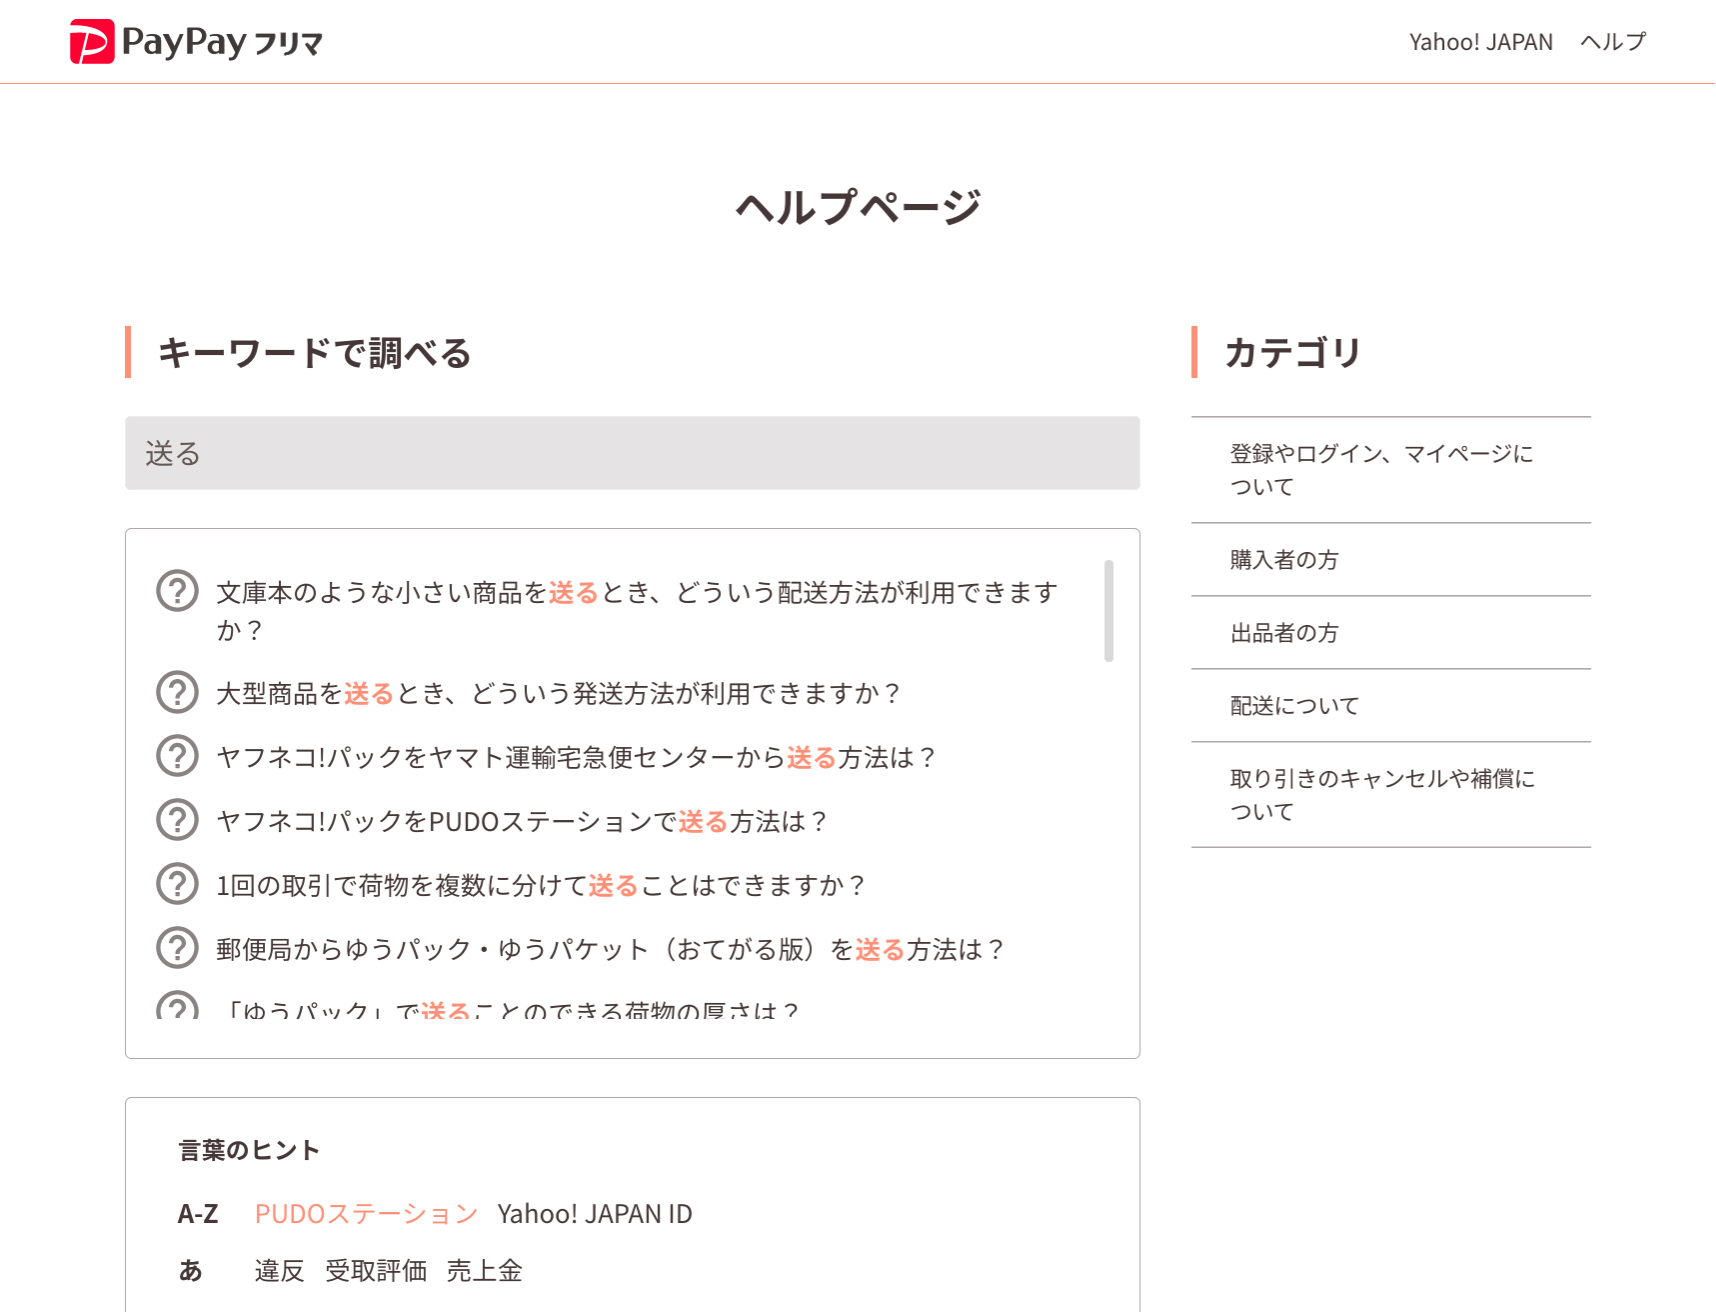
\includegraphics[width=10cm,bb=0 0 1716 1312]{figures/3d964512606a5e25646104a738ab104e.png}
  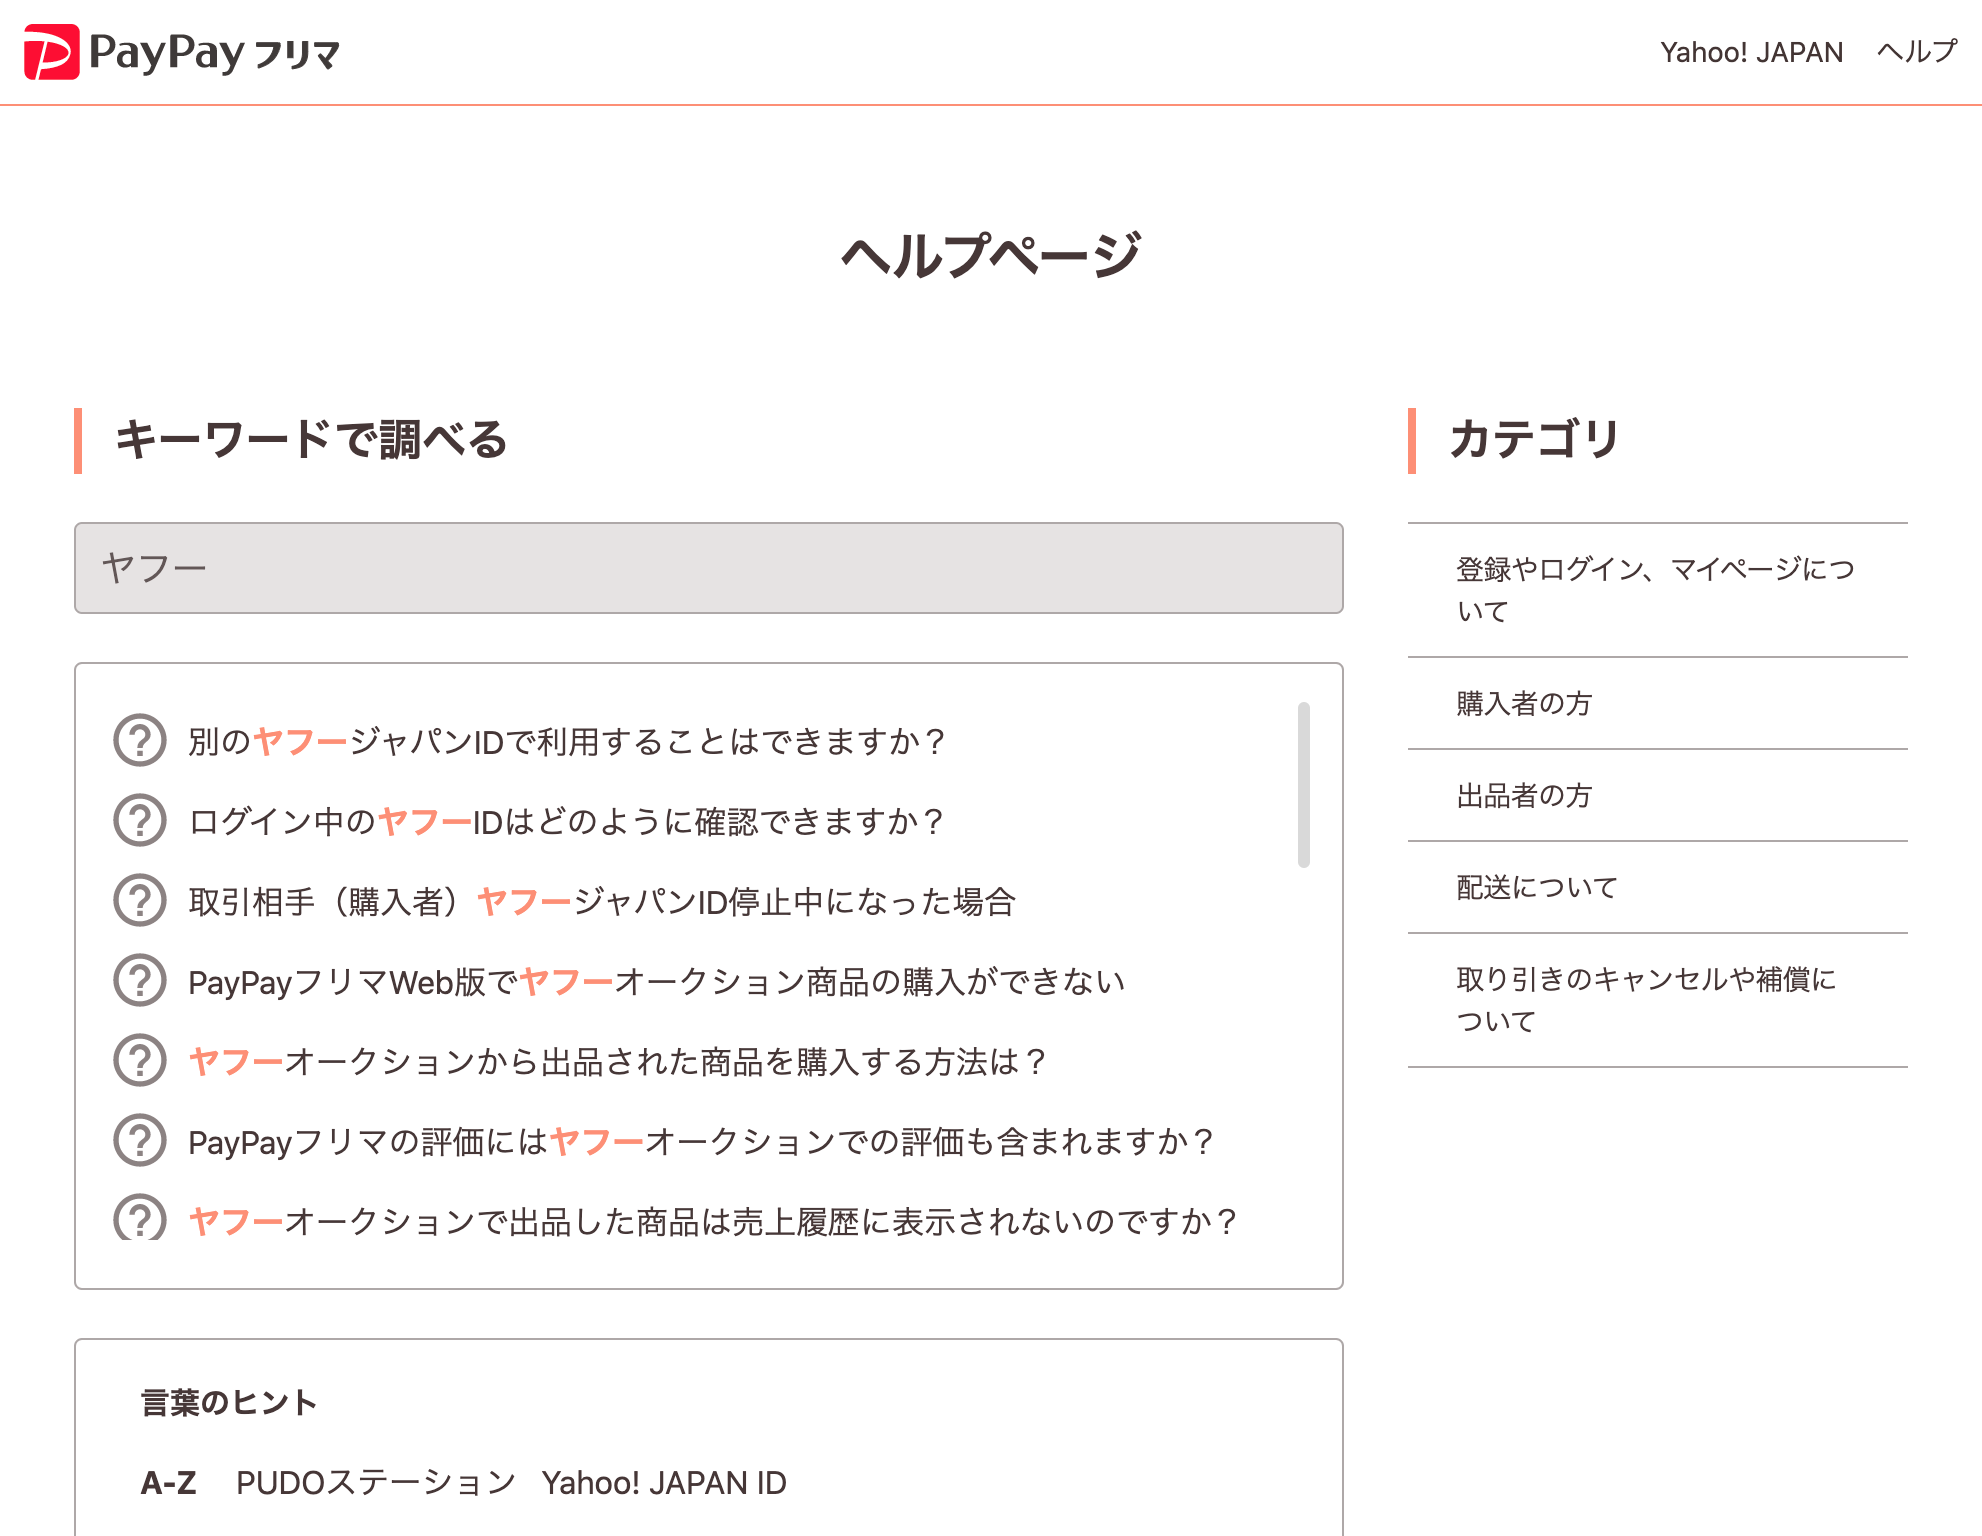
\includegraphics[width=7cm,bb=0 0 1982 1536]{figures/a0ba0873eeada33fad1bc383598f90c1.png}
  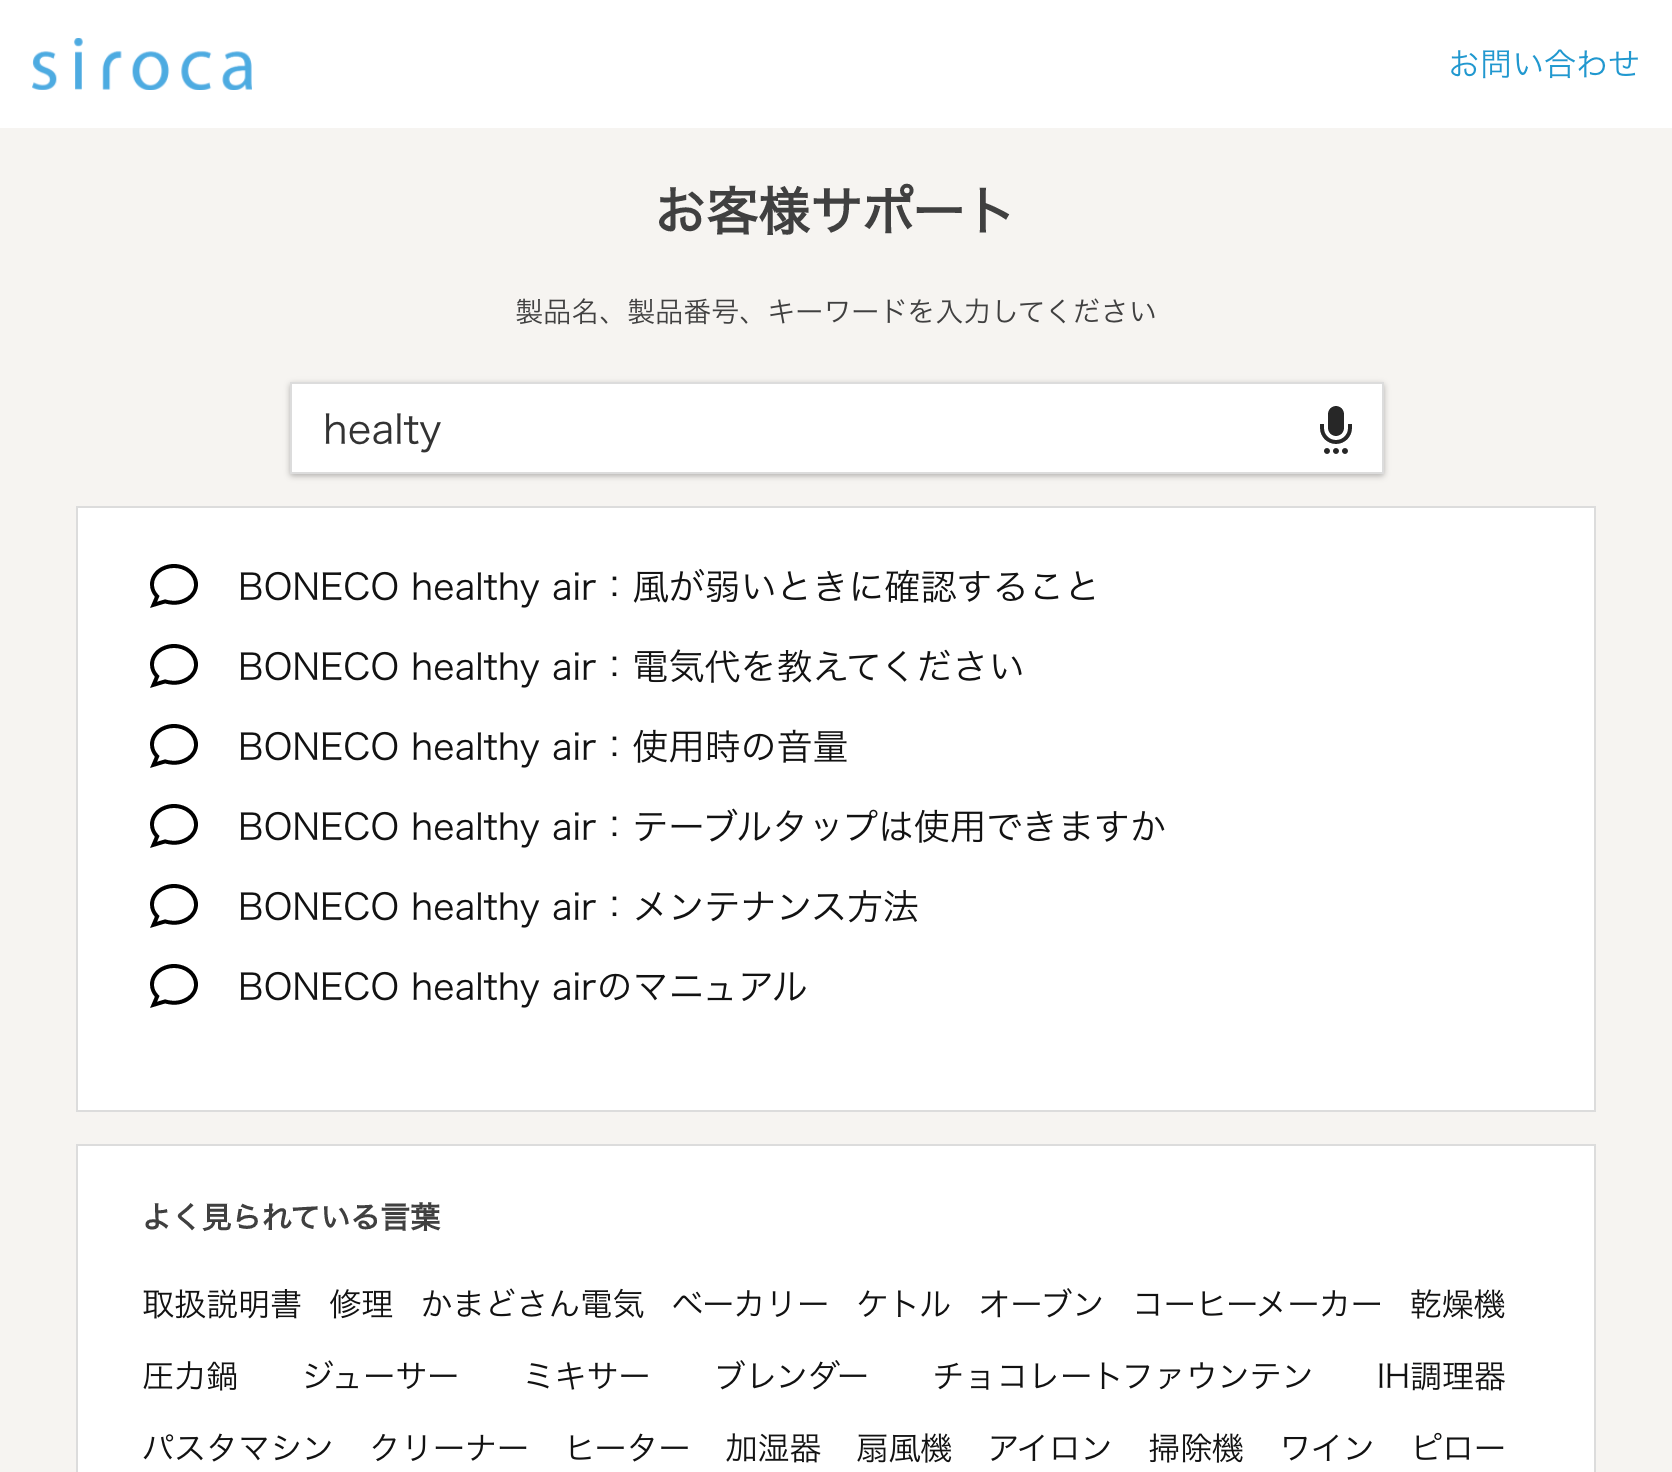
\includegraphics[width=7cm,bb=0 0 1672 1472]{figures/6b491f2701af7193030e332686733568.png}
  \caption{PayPay Freemarket}
  \label{paypayhf}
  %\Description{PayPay}
\end{figure}

After the introduction of ExpandSearch-based FAQ services,
the number of phone calls to the customer support center of these companies have
dropped to 40\%.
%
The ``hit rate'' at which users could find the information they need was 98\%.

\section{Implementation}

% [[実装]]
%  ExpandHelpのアルゴリズム
%   正規表現の拡張とパラメタ代入
%  HelpLineの実装
%   omniboxを利用するとか

\subsection{ExpandSearch}

A flexible search mechanism ``{\ES}'' is used in {\HL}.
%
The database used in {\ES} are provided as a set of data entries
consisting of a regular expression that represents description of the data entry
and a corresponding command pattern string.
A description string is used to produce natural language texts
that are easily understandable by users,
while command patterns represents the generated command string
corresponding to the description.
%
For example, a help entry for showing the difference between
current file and older file can be defined like this:

\begin{quote}
  \textbf{description}: \\
  \stt{Compare (\#\{files\}) with the one from (1|2|3|4) versions before}\\
  \textbf{command}: \\
  {\smallfont\verb|git diff $(git rev-list -n #{$2} HEAD -- #{$1})^ -- #{$1}|}
\end{quote}

Special symbols like \sqtt{\#\{files\}} in the description part is expanded to
the list of filenames like \sqtt{README.md|index.html}.
The first regular expression, the description part,
is for generating texts like
\sqsf{Compare README.md with the one from 1 versions before}, 
\sqsf{Compare index.html with the one from 2 versions before}, etc.,
and the second part, command part,
is used to generate a command to execute a {\GIT} command.
In the first example, \sqsf{README.md} and \sqsf{1}
match the first and second parentheses of the regular expression, and
these values are assigned to \tt{\$1} and \tt{\$2}
for the command part, generating a command
``{\smallfont\verb|$ git diff $(git rev-list -n #{$2} HEAD -- #{$1})^|}
{\smallfont\verb|-- #{$1}|}''.

The description part can be written in any natural language.
For example,

\begin{quote}
  \stt{(\#\{files\})を(1|2|3|4)個前のものと比較する}
\end{quote}
can be used for Japanese {\GIT} users.
In this case,
\sqsf{README.mdを1個前のものと比較する},
\sqsf{README.mdを2個前のものと比較する}, etc.
are used for the matching.

%% \subsection{(section written for GitHelp)}
%% 
%% {\EH} is a general-purpose flexible help generation system
%% that has the following characteristics.
%% 
%% \begin{itemize}
%% \item Use description-execution pairs for the translation
%% \item Standard regular expression is used for the specification of the description
%% \item The specification RegExp is expanded and filtered by the user's input string
%%   real-time
%% \end{itemize}
%% 
%% An example of the desc-exec pair can be the following:
%% 
%% \begin{verbatim}
%%   (delete|remove) a (#{file})
%%   /bin/rm $2
%% \end{verbatim}
%% 
%% ``remove \verb|README.md|''
%% into
%% ``\verb|rm README.md|
%% 
%% First, the spec like \stt{\#\{file\}} is expanded to a list of filenames like
%% \verb+README.md|Makefile|test.c+,
%% and the spec string becomes
%% ``\verb+(delete|remove) a file (README.md|Makefile|test.c)+''.
%% Then this regular expression is expanded to all the possible string that match this regexp like
%% \begin{verbatim}
%% delete a file README.md
%% remove a file README.md
%% delete a file Makefile
%% remove a file Makefile
%% ...
%% \end{verbatim}
%% 
%% And then all these strings are compared with the user's specification like
%% ``\verb|del REA|'',
%% and if a match is found,
%% this is translated to
%% ``\verb|delete file README.md|''.
%% 
%% If ``\verb|destroy|'' should also be used for the spec,
%% the spec can be modified to 
%% \stt{(delete|remove) a (\#{file})}.
%% 
%% Any kind of specs in any language can be used for the specification.
%% For example,
%% 
%% \begin{verbatim}
%%   \#{file}を(消す|消去する)
%%   /bin/rm $1
%% \end{verbatim}
%% 
%% can be  used for Japanese users, who might want to delete
%% one of the files by specifying ``消す''.
%% (消す means 'delete' in Japanese).

\subsubsection{Generating help menu entries}

Finding appropriate entries from the
% (possibly huge)
help document space is
performed in two steps.
First, a state transition diagram is generated from the regular expressions
used in the descriptions.
Second, all the description strings are generated by expanding the regular expression
into a tree, and filter the generated strings by the pattern specified by the user.
Efficient pattern matching is performed every time a new description text is generated,
and only the best-matched descriptions are shown to the user as menu entries.
We call this the ``\textit{generate-and-filter}'' technique,
and we will describe the details later.

\paragraph{Phase 1: Generating a state transition diagram from a regular expression}

Regular expressions are widely used for finding patterns in text strings
in modern programming languages and in the Unix environment.
In {\ES}, we use regular expressions for
generating various patterns of descriptions from a short specification.
For example, we use a short regular expression
\sqtt{(remove|delete|erase) (data|file)}
for representing expressions like
\sqsf{remove data},\sqsf{erase file}, etc.

Converting a regular expression to a state transition machine is a
straightforward task.
When we have a regular expression
\sqtt{Compare (README.md|index.html|package.json) with the one from (1|2|...|10) versions before}, 
we can convert it into a state transition diagram
shown in Figure \ref{statemachine1}.

\begin{figure}[htb]
\includegraphics[width=90mm,bb=0 0 571 126]{../../GitHelp/paper/figures/statemachine.pdf}
\caption{State transition diagram for a \stt{git} command description.}
\label{statemachine1}
\end{figure}

By traversing the nodes and links in this state machine,
we can generate the following description texts.

\begin{quote}
\small
\ssf{Compare README.md with the one 1 versions before} \\
\ssf{Compare index.html with the one 1 versions before} \\
...\\
\ssf{Compare package.json with the one 10 versions before}\\
\end{quote}

\paragraph{Phase 2: Generating texts from a state transition diagram}

Using the state transition diagram shown in Figure \ref{statemachine1},
{\ES} generates all the strings represented in the regular expressions,
and filter them by the pattern provided by the user.

We can generate texts from a state transition diagram by traversing nodes one by one.
Starting at the start node
\raisebox{-2pt}{\includegraphics[height=10pt,bb=0 0 40 40]{../../GitHelp/paper/figures/startnode.pdf}}
in Figure \ref{statemachine1},
we can visit other nodes via edges and generate a tree of generated texts
shown in Figure \ref{gentree1}.
After visiting the initial node
\raisebox{-2pt}{\includegraphics[height=10pt,bb=0 0 40 40]{../../GitHelp/paper/figures/startnode.pdf}},
the system generates a string \sqsf{Compare} and proceeds to the next node.
In the second generation,
the system can add \sqsf{README.md}, \sqsf{index.html}, and \sqsf{package.json}
to \sqsf{Compare}, generating
\sqsf{Compare README.md}, \sqsf{Compare index.html}, etc.
The system can repeat finding edges from previously visited nodes,
and eventually generates all the strings described above.
Of course, it is impossible to generate all the strings
from a regular expression like ``\tt{(0|1)+}'' that represents infinite length of
strings consisting of \tt{0}s and \tt{1}s, so the generation should be
terminated at a certain generation.

\begin{figure}[htb]
\includegraphics[width=85mm,bb=0 0 643 398]{../../GitHelp/paper/figures/gentree1.pdf}
\caption{Generating a text tree from a state transition machine.}
\label{gentree1}
\end{figure}

\subsubsection{Generate-and-Filter}

Generating all the texts in this way before finding matched strings is
inefficient, because the amount of generated texts can easily become huge.
Instead, the system performs the patter matching as soon as a text is generated,
for saving time and memory.

``Generate-and-test''\footnote{
  {\sf http:{\slash}{\slash}en.wikipedia.org{\slash}wiki{\slash}Generate\_and\_test}
}
is a simple and effective strategy used for solving puzzles.
For example,
the ``8-Queen'' problem can be solved simply by
generating all the possible queen layouts and checking if
two or more queens are laid out on the same row, column, or diagonal line.
Although this strategy is simple, the cost of
generating all the possible solutions is prohibitive, since
the solution space of the 8-Queen puzzle is $8^8 = 16,777,216$,
which is not a small amount even for today's computers.

To solve this problem,
controlling the generation part from the testing part is effective.
In the 8-Queen problem,
whenever the testing part finds two queens in the same row or column,
it can tell the generation part to
give up current layout in the early stage and proceed to the next layout.

Similarly in our case,
it is not efficient to perform the matching operation
after generating all the texts from the regular expression,
and it is better to calculate the matching
at the time of generating each text.
We call it the \qit{generate-and-filter} strategy,
and implemented the algorithm in {\ES}.
Unlike simple puzzle problems where
conditions are strict and finding one solution is enough,
our goal is to find help description strings
that fits the query pattern while allowing errors.
For this goal,
the system should perform approximate pattern matching
without sacrificing processing speed.
%
We could implement flexible generate-and-filter by using a simple and efficient
approximate pattern matching algorithm based on the ``shifter algorithm''.

\subsubsection{Approximate pattern matching by shifter algorithm}

The ``shifter algorithm''\cite{Wu:1992:FTS:135239.135244}
is a simple and efficient
text search algorithm that has interesting features
not found in more common pattern matching algorithms like
KMP\cite{KMP}, Boyer-Moor\cite{Boyer:1977:FSS:359842.359859}, etc.

When a user wants to find a word \sqsf{README} in a text,
he can use a patter matching state machine like below,
where the gray circle denotes that the state is active.

\begin{figure}[h]
  \centerline{\includegraphics[width=50mm,bb=0 0 439 73]{../../GitHelp/paper/figures/readme1.pdf}}
  \caption{A state machine for \qsf{README}.}
  \label{readme1}
\end{figure}

Initially, only the leftmost node is active, but when the
state machine receives \sqsf{R}, both the first and the second node become active,
and the activation state will change to the following pattern.

\begin{figure}[h]
  \centerline{\includegraphics[width=50mm,bb=0 0 439 73]{../../GitHelp/paper/figures/readme2.pdf}}
  \caption{After receiving \qsf{R}.}
  \label{readme2}
\end{figure}

When \sqsf{README} is given to the state machine,
the rightmost node becomes active.
%
%\begin{figure}[h]
%\includegraphics[width=60mm,bb=0 0 439 73]{figures/readme3.pdf}
%\caption{After receiving \qsf{README}.}
%\label{readme3}
%\end{figure}

Although this state machine is a nondeterministic finite state automata (NFA),
only 7 bits are required to represent the active/inactive states of the nodes,
meaning that the whole states can be represented by a single integer value.
Also,
the state transition can be calculated by a simple combination of
logic and bit shift operations.

\subsubsection{Approximate pattern matching using shifter algorithm}

The state machine shown in Figure \ref{readme1} can accept only one pattern
(\sqsf{README}), but
it can be easily expanded to detect texts that contain a word
similar to the pattern (e.g. \sqsf{REEDEE}).

% \begin{figure}[htb]
%   \centerline{\includegraphics[width=30mm,bb=0 0 104 51]{figures/readme-mismatch.pdf}}
%   \caption{Matching error between \qsf{README} and \qsf{REEDEE}.}
%   \label{readme-reddy-mismatch}
% \end{figure}

Adding three more rows of states to Figure \ref{readme1}, we can perform more
flexible pattern matcher which can accept strings with
0 to 3 matching errors.

\begin{figure}[htb]
  \centerline{\includegraphics[width=60mm,bb=0 0 443 282]{../../GitHelp/paper/figures/readme-ambig.pdf}}
  \caption{A pattern matcher accepting 0-3 errors.}
  \label{shifterambig}
\end{figure}

Figure \ref{shifterambig} shows a state machine that can detect a string
that matches \sqsf{README} with 0 to 3 mismatches.
Each additional row of nodes represents a matcher with one error,
two errors, and three errors, respectively.
Vertical and diagonal transition edges are added to allow
transitions based on spelling errors.

Initially, only the bottom-left node is active.
When a character other than \sqsf{R} is detected, 
the transition labeled \sqsf{*} (wildcard) is activated,
and connected nodes become active.
At the same time, links labeled as ``$\epsilon$''
is also activated without any input character.
With these additional links, this expanded machine can detect a text which
matches \sqsf{README} with 0 to 3 errors.

\begin{figure}[htb]
  \centerline{\includegraphics[width=60mm,bb=0 0 443 282]{../../GitHelp/paper/figures/readme-reedee.pdf}}
  \caption{Accepting \sqsf{REEDEE}'' using a matcher for \sqsf{README}.}
  \label{readme-reedee}
\end{figure}

The transition of active nodes while reading
\sqsf{REEDEE} is shown in Figure \ref{readme-reedee}.
After reading \sqsf{REEDEE},
only the upper-right node becomes active,
denoting that \sqsf{REEDEE} matches
\sqsf{README}'' with 2 matching errors.

The state transition shown in 
Figure \ref{readme-reedee} looks complicated, but
the matching state can be represented by only four integer variables, and
the matching algorithm can be implemented efficiently.

\subsubsection{Using the matcher for generate-and-filter}

We can use this approximate pattern matcher while generating
help texts by traversing the state transition machine.
%
Every time a new node is generated by traversing an edge,
matching state is calculated and stored in the generated node.
The status pattern is calculated from the status pattern
stored in the preceding node and the string associated with the edge.

\begin{figure}[htb]
  \centerline{\includegraphics[width=50mm,bb=0 0 302 230]{../../GitHelp/paper/figures/RE_2.pdf}}
  \caption{A pattern matcher for \sqtt{REE 2}.}
  \label{RE_2}
\end{figure}

\begin{figure*}[bth]
\centerline{\includegraphics[width=110mm,bb=0 0 643 446]{../../GitHelp/paper/figures/gentree2.pdf}}
\caption{Matching statuses for \sqtt{REE 2} associated with text generation nodes.}
\label{gentree2}
\end{figure*}

Figure \ref{RE_2} shows the matcher for \sqtt{REE 2}\footnote{
  A space (\qtt{ }) in the input is treated as a wildcard character.
},
and Figure \ref{gentree2} shows how the matching status is calculated while the
description strings are generated from the state transition machine
shown in Figure \ref{statemachine1}.
The matching status at each node is calculated from the matching status
stored in the parent node and the string associated with the edge.
For example, when the system generates the string
\qsf{Compare README.md with the one from 2 versions before},
the matching status is calculated from the status data at the previous node at
\qsf{Compare README.md with the one from 2}, and
the system can tell that it matches \qtt{REE 2} with one matching error,
as soon as the string is generated.

The system is keeping the list of generated strings
which match the pattern with zero to three errors
and it displays the list with minimal number of errors
when generating menu entries.
% 
Since the pattern matching operation is performed at the time of text generation,
the whole generate-and-filter calculation is quick.

% Although current version of ExpandHelp is implemented in MacRuby,
% the user can always get the result within 1 second.
% A portion of the help data in Ruby is shown in Figure \ref{helpdata}.

% \begin{figure*}[bt]
% \centerline{\includegraphics[width=146mm]{../../GitHelp/paper/figures/04ad7dee5679450e5390821745b5a0b7.png}}
% \caption{A portion of the help data in Ruby.}
% \label{helpdata}
% \end{figure*}

\subsection{Sharing the database on the Web}

The data used in {\HL} are represented as ``{\SB}'' documents
shown in Figure \ref{scrapboxpage}.
%
{\SB} is a general-purpose real-time Wiki system for data sharing.
{\SB} users can edit the contents of Wiki pages directly
on Web browsers just like using text editors.

% \begin{figure}[htb]
% \begin{verbatim}
% \end{verbatim}
% % \centerline{\includegraphics[width=100mm,bb=0 0 1428 1288]{../../GitHelp/paper/figures/scrapbox1.png}}
% \centerline{\includegraphics[width=100mm,bb=-50 -50 1000 900]{../../GitHelp/paper/figures/scrapbox1.png}}
% \caption{A {\SB} page for \tt{git diff}.}
% \label{xxxxx}
% \end{figure}

This page shows how to use \sqtt{git diff}, and
the page contains command specifications in {\ES} format
in addition to the documentation.

% Specs and command lines are specified with a special symbol, and
% all other documents can be written just like standard manuals and help documents.

Usage examples are often shown on documents and manuals like Unix man pages,
but they cannot be used as the database of an online help system.
On the other hand,
a {\SB} document contains both the manual document and the help database
in the same place, just like
writing a source code and the document in the same place
under the ``Literate Programming''\footnote{
  \ssf{https:{\slash}{\slash}en.wikipedia.org{\slash}wiki{\slash}Literate\_programming}
} style.

Also, since the database is on the Wiki page, any member of the
Wiki can correct the document or add additional {\HL} specifications.
When a user could not get a good support from {\HL}, he can add
{\ES} specifications to the {\SB} document himself
so that he and other people can get better support
from {\HL} next time.

\section{Related Work}

\subsection{Intelligent help systems}

There have long been many researches on
intelligent help systems\cite{Delisle:2002:UIH:606412.606415},
but few number of projects seem to be going on these days,
maybe because now we can use the Internet for getting intelligent help from
real people,
either by searching existing Web pages or 
by asking in user forums like StackOverflow\footnote{
  \ssf{https:{\slash}{\slash}stackoverflow.com{\slash}}
}.
Information on the net is rich these days, and we can easily
find somebody who can give good answers to our questions.
This is a good news, but 
asking many trivial questions on the net is not considered to be a
good manner, and
using a powerful and flexible local help system like {\ES} is
preferable most of the time.

\subsection{Input Methods}

Text input systems for non-English languages are widely used
in the world,
and they are called as ``Input Methods'' (IMs).
%
Many research and development on IMs have been going on for years, and
people are using them every day for entering texts in their mother language.
Figure \ref{gyaim} shows an example of a Japanese IM.

\begin{figure}[H]
  % \includegraphics[width=8cm,bb=0 0 976 670]{../../GitHelp/paper/figures/nyuuryoku-ime.png}
  \centerline{\includegraphics[width=8cm,bb=0 0 976 670]{../../GitHelp/paper/figures/nyuuryoku-ime.png}}
  \caption{An IM for Japanese text input.}
  \label{gyaim}
\end{figure}

IMs are one form of translation systems that convert one
expression (pronunciation, character shape, etc.)
into a textual form of a language.
In the above example, the pronunciation ``kanji''
is used for getting ``漢字''.

IMs are very popular in the modern computing environment in the world
and it is very common for people to 
use translation systems for using computers.
%
The behavior of {\HL} is similar to conventional IMs, and
integration of multiple IM-like systems should be challenged in the future.

\subsection{Text and code completion}

On text editors and Unix shells,
``text completion'' feature has been available for a long time.
%
When a user types the TAB key after typing \sqtt{la} on the Unix shell,
\sqtt{latex}, \sqtt{last}, and other Unix commands are shown as candidates.
When a user types \sqtt{ls RE} and types the TAB key,
the shell checks the directory, find the \stt{README.md} file, and
replace the user's input with \sqtt{ls README.md}.
This behavior is called ``text completion'', and many variations of
this idea have been proposed and adopted in command shells and text editors.

% User's history data can also be used for the completion function.
% The Reactive Keyboard\cite{ReactiveKeyboard}
% accumulates the user's command history and use the data
% for predicting the user's next input.

Gitsome\footnote{\textsf{https:{\slash}{\slash}github.com{\slash}donnemartin{\slash}gitsome}}
helps {\GIT} users by
dynamically showing possible arguments and related manuals on the Unix shell,
just like {\HL} does.
The goal of Gitsome is almost the same as {\HL} and we agree with its concept,
but Gitsome does not support flexible approximate matching and
help data sharing.

\subsection{Smart IDEs}

Integrated Development Environments (IDEs) are widely used for
software development, and
many smart IDEs for suggesting codes have been proposed recently.

Little's system\cite{Little:2006:TKC:1166253.1166275}
generates a complete JavaScript code snippet from keyword fragments
give by users.
For example, a code snippet
\sqtt{ActiveDocument.PageSetup.LeftMargin = InchesToPoints(2)}
can be generated from keywords like
\sqsf{left},
\sqsf{margin},
\sqsf{inches},
and \sqsf{2}.
The system generates the code using a template database and heuristics
designed for the target system.
It is useful for a specific environment, but
users of the system cannot modify the algorithm or the database
even when no good suggestion was found.

% キーワードの羅列からコマンドを作成するという考えはとても正しいと思うが、実装がいかがなものか?
% キーワードぐらいは思い出せるプログラマが対象になっている
% 「margin」とか「left」とかいう単語は思い出す必要がある
% 「ちょっと字下げ」とか言っても駄目
% キーワードが違ってると駄目?
% いろいろズルをしてるようだ
% [[ActiveDocument]]はよく出てくるので特別扱いしているとか
% ステミングをしている
% ``the'' ``to'' などは捨ててるのだろう
% そもそもリカーシブな検索アルゴリズムにかなり無理がありそう
% テンプレートを作るのは大変ではないのか?

% https://www.youtube.com/watch?v=93vZAmLyOQY
AnyCode\cite{Gvero:2015:SJE:2814270.2814295} is another system
that generates a complete code snippet from the user's
input in natural language.
AnyCode can handle synonyms database like ``make'' == ``create'',
but approximate matching is not supported and
users cannot modify the help database.

% 曖昧検索はできず、かなりキーワードを指定する必要はある

% [anyCode]というシステム。自然言語キーワードを入力するとコードスニペットが表示される。
% [[copy fileA fileB]]みたいなキーワードから[[FileUtil.copyFile(new File(fileA), new File(fileB))]]みたいなコード候補を生成する
% [自然言語処理]を行なっている
% [https://github.com/tihomirg/nlpcoder/tree/noola GitHub]
% 曖昧検索はできない
% 真面目に自然言語を入れる必要がある
% `123`みたいなパラメタは使えるか?
% 使えると思うが例には出てこない
% コードの説明文は出ない?
% FileUtil.copyFile(new File(fileA), new File(fileB)) と言われても、どちらが新しいファイルなのかわからない

Active Code Completion\cite{Omar:2012:ACC:2337223.2337324}
is another code completion system for the Eclipse IDE.
A database called \textit{palette} are used for code completion and coding support
for Java classes.
When a user wants to write a code for drawing a rectangle in purple,
the user should just tell ``purple'' to the system,
and the system shows the user a color selection window
as well as the Java code for drawing a purple rectangle.
This is a useful feature for the user to write a code including selecting
a color, but palettes are difficult to create, and should be provided
as IDE plugins.
% [/ palette] と呼ばれるテンプレートを用意して[IDE]でのコード補完をサポートする
% `getDefaultColor()` を定義したいとき`purple`と入力すると、それに対応した候補が提示されるとか
% 普段使ってる環境で有益な候補が表示されると嬉しいだろうと言っている
% [[コメント]]
% [Jun Kato.icon]
% > Active code completionも思い出しました。型ごとに適した入力インタフェースを出すコード補完インタフェースのnn提案です。確か。
% [増井俊之.icon]
% IDEでどういう機能が欲しいかサーベイして設計したことになっている
% 色選択と正規表現のためのコード生成をサポートした例が紹介されている
% 一般的な補完コマンド起動によって呼び出されるようだ
% サポートウィンドウはHTML5で生成する
% しかし両者とも[/palette]の作成はかなり大変である
% 普通のユーザが作れるようなものではない
% [* 作成がすごく大変]で、[* 特定のIDEでしか使えない]という問題があると思う

Han's Abbreviation Completion system\cite{Han:2009:CCA:1747491.1747530}
can generate a code snippet from abbreviation strings give by the user.
For example, a code snippet like \sqtt{chooser. showOpenDialog()}
can be generated from strings like
\sqsf{ch} and \sqsf{opn}, using the code database and HMM.
It can be very useful as a shorthand for handling long names,
but users should have a vague knowledge about the correct names
(e.g. \sqtt{chooser}, \sqtt{dialog}),
and large code example corpus should exist before being able to
create the database.
{\ES} database can be created by hand at the time of the system development
and no corpus is required.

% [HMM]を使って正しいコードを予測して提示する
% `ch opn`みたいなテキトーな入力から`chooser.showOpenDialog()`みたいな正しいコードが候補に出る
% コードデータベースを解析
% [[コメント]]
% [増井俊之.icon] 2018/3/23 18:53
% コードのほんの一部を指定すると正しく予測されるというのは面白い
% HMMってそういうのに使えるのね
% しかし[* 関数名とか全然覚えていないときは使えないだろう]
% [語彙問題]が解決できてない
% だとすると高速入力の役にはたつが、何もかもわからない人をサポートはできない
% 用例データが存在しない場合も使えない
% [IDE]でしか使えない
% [Cyrus Omar: Active code completion]で参照されている

\subsection{Using cloud data for development}

% 他人の情報利用する系
% コード共有、コンパイルエラー共有

Many systems support sharing users' development experiences on the web so that
they can be used on the developers' IDE.

Using BluePrint\cite{Brandt:2010:EPI:1753326.1753402}
as a plugin for Adobe Flex Builder,
users can search sample codes from the Web and use it immediately.
%   サンプルコードをすぐ参照して利用できる[IDE]
%
HelpMeOut\cite{Hartmann:2010:OPS:1753326.1753478} tells users
how to handle compile errors,
based on the people's experiences of handling compile errors.
%
Resources on the net are precious, and such data can be
easily incorporated to {\ES} databases.

%= 他人のヒストリを使ってコンパイルエラー対処法をサジェスト

% \subsection{Literate Programming}
% 
% Literate Programming\cite{Knuth}
% 
% 参考文献にすることはないか
% 
% JavaDoc
% Jupyter
% Eve

\section{Discussions}

%     検索システムを選んでから検索キーワードを入力するのに慣れてしまっている
%   この必要がないことを知ると驚きがある
%  検索されやすいように工夫するとか馬鹿げてると
% 思うかもしれないか、ググって出なきゃ無いのと同じだということを考えると、
% ある程度工夫することは意味があるし、自分が後でさがすときにも役に立つわけである
%   ゲームのように記述を増やす工夫もできるかもしれない
%   タイトルに迷ったら両方書くみたいな
%  どこにある情報でもひとつのインタフェースでみつかるのは強烈に嬉しい
% 
% [[説得ポイント]]
%  ExpandHelp
%   自分が入力したキーワードが検索結果に出現する嬉しさ
%  検索方法の統合
%  ヘルプシステムの実績
% 
% [[関連システム / 参考文献]]
%  普通の[https://en.wikipedia.org/wiki/Query_expansion クエリ拡張]
%  Relevance Feedback
%   検索パタンを増やすことに効果があるといえる
%  [https://scrapbox.io/UIPedia/George_Furnas:_The_vocabulary_problem_in_human-system_communication Vocabulary problem]
%  [文芸的プログラミング]
%   ExpandHelp記述は文芸的プログラミングの一種だと思えばいい
%   冗長な感じで書くといい
%  [/Rubytips] の実例
% 
% 日本語を入力すると英語のWikipediaがみつかることもある
%  これはたぶん原文を翻訳したものを検索対象にしている
%  これもDocument Expansionといえる

\subsection*{Other applications of ExpandSearch}

Since the translation mechanism of {\ES} is simple and flexible,
it can be used for a wide range of application domains where
intelligent help is required.
{\ES} is actually used as the help page for
one of our Web services, hoping that
novice users can easily find the feature they need.
When a user submits a query that includes vocabularies
not in the {\ES} document,
we are able to add them to the {\SB} database easily.

Figure \ref{mac1} and Figure \ref{mac2} shows how
{\ES} can be used as a launcher for MacOS.
Like {\HL}, users can execute concrete commands only by
showing small fragments of their intentions to the system.

\begin{figure}[h]
  %\centerline{\includegraphics[width=8cm,bb=0 0 397 247]{../../GitHelp/paper/figures/clock.png}}
  \centerline{\includegraphics[width=7cm,bb=0 0 300 200]{../../GitHelp/paper/figures/mac1.png}}
  \caption{Using {\ES} in the menu bar of MacOS.}
  \label{mac1}
\end{figure}

\begin{figure}[h]
  %\centerline{\includegraphics[width=8cm,bb=0 0 392 185]{../../GitHelp/paper/figures/mac2.png}}
  \centerline{\includegraphics[width=7cm,bb=0 0 300 130]{../../GitHelp/paper/figures/mac2.png}}
  \caption{Using {\ES} in the menu bar of MacOS.}
  \label{mac2}
\end{figure}

\subsection*{Order of command and arguments}

Using a command shell,
users have to enter a command first and enter options and arguments after that.
Using a GUI desktop,
users can right-click a data icon to show a menu,
and select what he wants to do from the menu.
Switching between command-oriented usage pattern and
data-oriented usage pattern is sometimes confusing.
Using {\ES}, users can find what they can do
either by specifying commands or by specifying data, 
without worrying about the order.

\subsection*{Usage of regular expressions}

An advantage of using a regular expression is that
it is fairly easy for users to write description texts.
People can easily write a help description like
\sqtt{(Start|Run) Firefox browser}
without having a knowledge of automata or formal grammar.
We can use arbitrary texts for the database of {\ES}.
For example,
we can collect hundreds of books titled ``Windows tips'' from the market
and convert all the title of the tips into help data of {\ES}.

\section{Conclusion}

We proposed the ``translation paradigm'' for bridging the gap between
users' intention and actual operations.
%
We have introduced a general-purpose flexible framework {\ES}
that can translate fragments of user's vague intentions into
concrete command strings required to control computers and
other complex artifacts.
We showed the principles and applications of {\ES} by using it
for {\HL}, a help system for supporting {\GIT} users
based on the shared database that any user can edit to share
translation knowledge between users.
%
{\ES} framework is useful for any kind of systems that need
some kind of user support, and we are planning to use it
for various applications and Web services in the future.

% Unlike existing smart IDEs for supporting programming tasks,
% {\ES} framework can be used in wide range of situations
% where translation-based help is required.
% 
% Using the powerful and flexible help system ``{\ES}''
% constructed on the generate-and-filter algorithm, where
% the system generates all the possible expressions of
% help entries expanded from regular expressions,
% while the output expressions are filtered by search keywords using
% an efficient approximate pattern matching algorithm.
% 
% Since the data format is simple and the search algorithm is fast and flexible,
% developers can easily publish useful help data, while
% users can have bigger chances of finding an appropriate
% data from vague knowledges.

% References must be the same font size as other body text.

\newpage

\bibliographystyle{ACM-Reference-Format}
\bibliography{paper}


\end{document}


% \endinput

